% Gershgorin discs (rows) of a 4x4 complex matrix, with its eigenvalues (dots). Eigenvalues: 4.110+0.026i, 1.239+0.230i, -1.103+0.982i, -0.245+1.262i
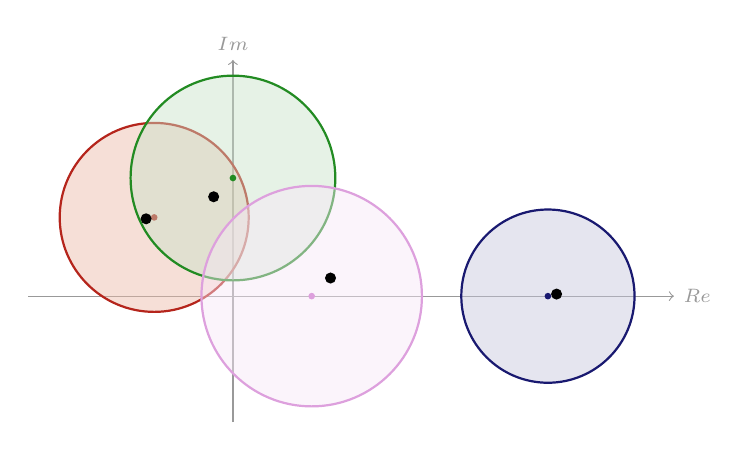
\begin{tikzpicture}[scale=1.00]
\draw[->,black!40] (-2.6,0) -- (5.6,0) node[right,font=\scriptsize] {$\operatorname{Re}$};
\draw[->,black!40] (0,-1.6) -- (0,3.0) node[above,font=\scriptsize] {$\operatorname{Im}$};
\fill[MidnightBlue!25,opacity=0.45] (4.000,0.000) circle (1.100); \draw[MidnightBlue,thick] (4.000,0.000) circle (1.100);
\fill[MidnightBlue] (4.000,0.000) circle (1.2pt);
\fill[BrickRed!25,opacity=0.45] (-1.000,1.000) circle (1.200); \draw[BrickRed,thick] (-1.000,1.000) circle (1.200);
\fill[BrickRed] (-1.000,1.000) circle (1.2pt);
\fill[ForestGreen!25,opacity=0.45] (0.000,1.500) circle (1.300); \draw[ForestGreen,thick] (0.000,1.500) circle (1.300);
\fill[ForestGreen] (0.000,1.500) circle (1.2pt);
\fill[Plum!25,opacity=0.45] (1.000,0.000) circle (1.400); \draw[Plum,thick] (1.000,0.000) circle (1.400);
\fill[Plum] (1.000,0.000) circle (1.2pt);
\fill[black] (4.110,0.026) circle (2pt);
\fill[black] (1.239,0.230) circle (2pt);
\fill[black] (-1.103,0.982) circle (2pt);
\fill[black] (-0.245,1.262) circle (2pt);
\end{tikzpicture}
